\documentclass[crop,tikz]{standalone}
\usetikzlibrary{backgrounds}
\colorlet{blue}{cyan}
\tikzset{
  inverted/.style = {
    color=white,
    background rectangle/.style={fill},
    show background rectangle
  }
}

\usepackage{pgfplots}
\pgfplotsset{compat=1.16}
\usepgfplotslibrary{colormaps}
 
\begin{document}
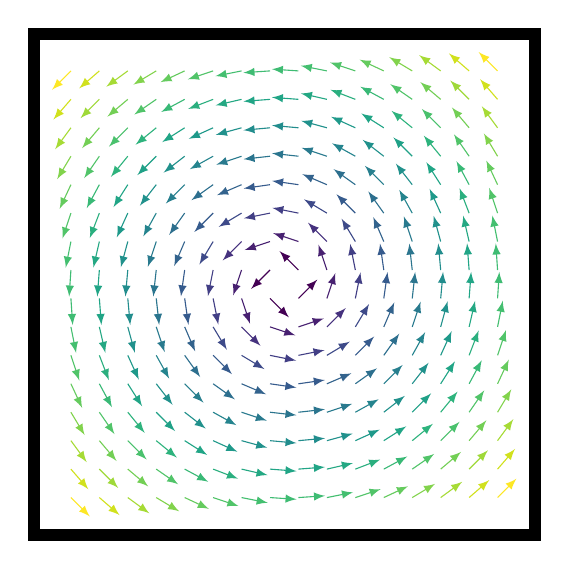
\begin{tikzpicture}[inverted,inverted]
\begin{axis}[inverted,
  xmin = -2, xmax = 2,
  ymin = -2, ymax = 2,
  zmin = 0, zmax = 1,
  axis equal image,
  height=7cm,
  view = {0}{90},
  colormap/viridis,
  xtick={\empty},
  ytick={\empty},
  hide axis,
  samples = 16,
  clip=false,
  ]
  \addplot3[
    point meta = {sqrt(x^2+y^2)},
    quiver = {
      u = {-y/sqrt(x^2+y^2)},
      v = {x/sqrt(x^2+y^2)},
      scale arrows = 0.25,
      every arrow/.append style={
        -{latex[scale={max(0.7,\pgfplotspointmetatransformed/1000)}]},
      },
   },
   domain = -2:2,
   domain y = -2:2,
   quiver/colored = {mapped color},
  ] {0};
\end{axis}
\end{tikzpicture}
\end{document}
